\documentclass[10pt,a4paper,titlepage]{article}
\usepackage[latin1]{inputenc}
\usepackage{amsmath}
\usepackage{amsfonts}
\usepackage{amssymb}
\usepackage{blkarray}
\usepackage{graphicx}
\usepackage{appendix}
\usepackage{listings}
\usepackage{biblatex}
\usepackage{hyperref}

\bibliography{refs.bib}
\usepackage{color}
\definecolor{dkgreen}{rgb}{0,0.6,0}
\definecolor{gray}{rgb}{0.5,0.5,0.5}
\definecolor{mauve}{rgb}{0.58,0,0.82}

\lstset{ %
  language=Octave,                % the language of the code
  basicstyle=\footnotesize,           % the size of the fonts that are used for the code
  numbers=left,                   % where to put the line-numbers
  numberstyle=\tiny\color{gray},  % the style that is used for the line-numbers
  stepnumber=1,                   % the step between two line-numbers. If it's 1, each line 
                                  % will be numbered
  numbersep=5pt,                  % how far the line-numbers are from the code
  backgroundcolor=\color{white},      % choose the background color. You must add \usepackage{color}
  showspaces=false,               % show spaces adding particular underscores
  showstringspaces=false,         % underline spaces within strings
  showtabs=false,                 % show tabs within strings adding particular underscores
  frame=single,                   % adds a frame around the code
  rulecolor=\color{black},        % if not set, the frame-color may be changed on line-breaks within not-black text (e.g. commens (green here))
  tabsize=8,                      % sets default tabsize to 2 spaces
  captionpos=b,                   % sets the caption-position to bottom
  breaklines=true,                % sets automatic line breaking
  breakatwhitespace=false,        % sets if automatic breaks should only happen at whitespace
  title=\lstname,                   % show the filename of files included with \lstinputlisting;
                                  % also try caption instead of title
  keywordstyle=\color{blue},          % keyword style
  commentstyle=\color{dkgreen},       % comment style
  stringstyle=\color{mauve},         % string literal style
  escapeinside={\%*}{*)},            % if you want to add a comment within your code
  morekeywords={*,...}               % if you want to add more keywords to the set
}

\author{Wouter ibens \\ University of Antwerp}
\title{The power of two paths in grid computing networks}
\begin{document}
\maketitle

\section*{Abstract}
a

\newpage

\tableofcontents

\newpage

\section*{Introduction}
Write at the end


\section{Setup}
We are using a ring-structured network of $N$ nodes. Each node is connected to two neighbours, left and right. The purpose of these nodes is to process incoming jobs. When a node is busy while a job arrives, it must forward to another node. When a job has visited all nodes and none of them was found empty, the job is dropped.

Jobs have an arrival time, a length and optional metadata. They arrive at each node indepentently as a poisson process at rate $\lambda$. Their length is exponentially distributed with mean $\mu$ (unless otherwise noted, assume $\mu=1$). Although each job has a length, this length may not known in advance. Finally, the metadata is optional and may be used by the nodes to pass information among the job (e.g. a list of visited nodes).

Nodes can use different algorithms to determine whereto a job will be forwarded. The performance of these algorithms is the main focus of this thesis. Different techniques will be discussed and simulated. Afterwards, some results of the simulation will be validated.
Note that the cost of forwarding a job is neglected. Together with the presumption a job must visit each node before being dropped, this means a job arriving at any node will be processed if and only if at least one server is idle.

\begin{figure}[h!tb]
\centering
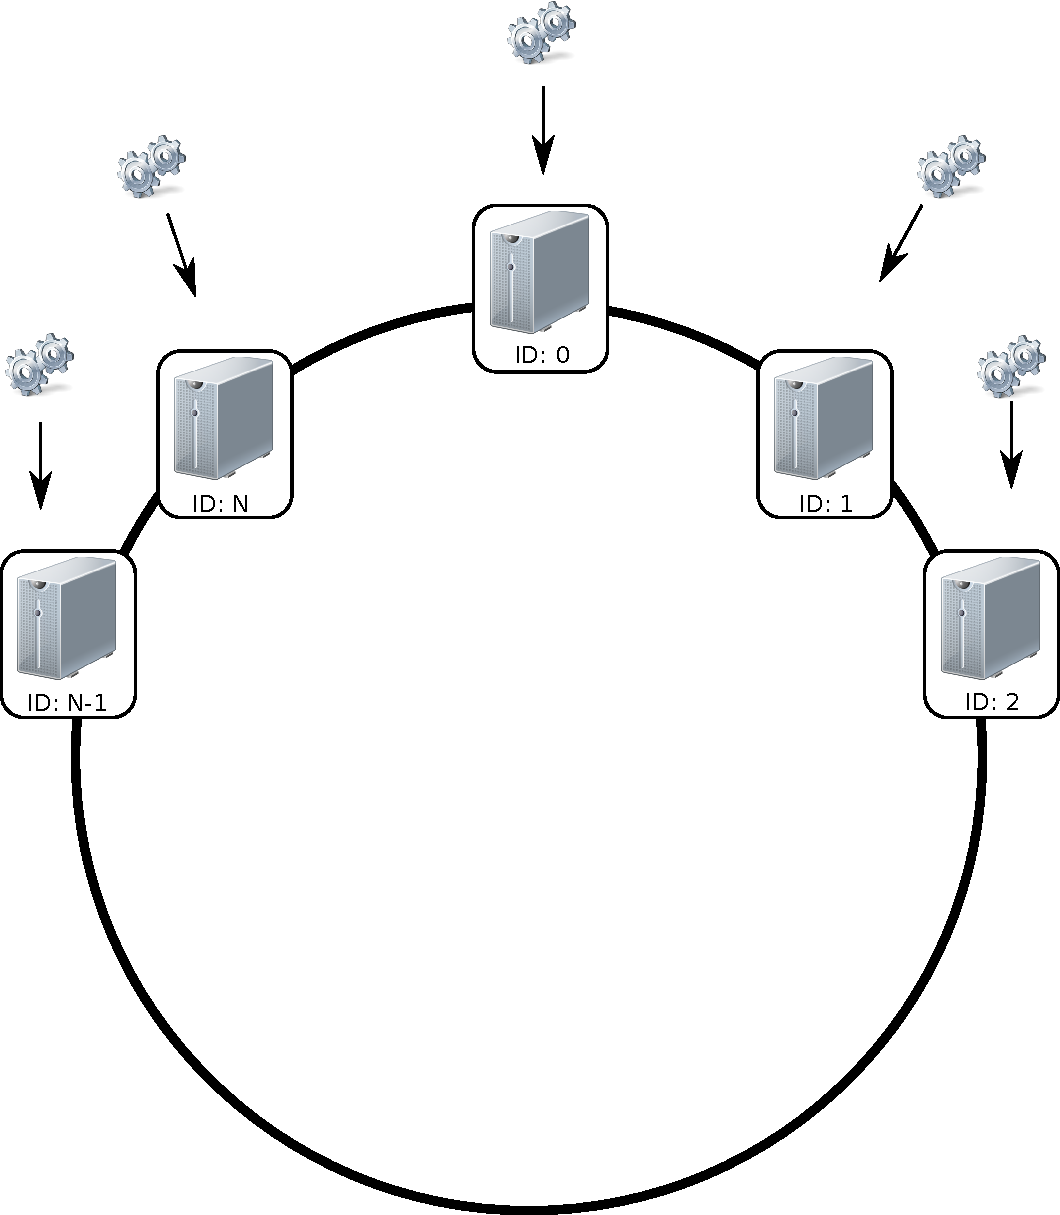
\includegraphics[width=0.8\textwidth,clip=true,trim=0px 225px 0px 0px]{resources/ring.pdf}
\caption{A ring structured network}
\label{figring}
\end{figure}

The performance of a forwarding algorithms is measured by the average number of hops a job must visit before being executed. The goal of the algorithms is to minimize this number by spreading the load evenly along the ring. 


%Explain the setup, the goals, the reasons, explain the balancing-techniques
%Insert a picture of nodes in a ring
%
%Imagine a ring-structured distributed system, consisting of several nodes, each connected its two neighbours. Nodes may have $x$ servers, meaning they can process at most $x$ jobs at a time. External jobs will arrive at each node, independent of eachother. Busy nodes will pass an incoming job on to another node using a specified algorithm. This setup is fixed during the whole thesis. Our goal is to examine how well given algorithms distribute the load of the system. It is measured using the average number of times a job must be forwarded before is can be executed. Jobs that are forwarded to every node in the system are discarded. We assume the jobs have a Poisson arrival rate with parameter $\lambda$, the service time is exponental with parameter $\mu$, and forwarding a job takes no time at all. Unless otherwise noted, we assume $\mu=1$.

\subsection{Forwarding algorithms}
Nodes that must forward a job must choose another node of the ring. Nodes have no information about other nodes, so is has no idea whether the node is idle or busy. The algorithms are grouped in two categories: forward to neighbour and forward anywhere.
The first techniques allows a busy node to forward an incoming job to either its left or right neighbour, where the latter may forward these jobs to any node in the ring. 
Since the amount of dropped jobs is equal for each forwarding algorithm. These jobs will be ignored when computing the average number of hops.


\subsection{Forward to neighbour}
\subsubsection{Forward right}
A busy node using this technique will forward a job to its right neighbour. The job will keep travelling clockwise until an idle node is found, where it will be processed. This algorithms is used as base line in all further tests.

\subsubsection{Left/Right forward}
A variant to the previous algorithm is the Left/Right forward technique. Instead of forwarding each job to its right neighbour, a busy node will alternate the direction after forwarding such a job. To avoid a job coming back, this initial direction is saved in the job's metadata. Busy nodes receiving a job from another neighbour must forward it the same direction as specified in the job's metadata.

\subsubsection{Random Left/Right forward with parameter $p$}
This technique is a variant of the Left/Right forward algorithm. However, instead of alternating the direction for each new job, a node will forward a job to its right with probability $p$ and to its left with probability $1-p$. As the previous technique, the direction is saved in the job's metadata and subsequent nodes must maintain this direction when forwarding.

\subsubsection{Position-dependant forwarding}
As shown in figure \ref{figring}, each node in the ring has an unique ID. Except the for node with id $0$ and $N-1$, neigbouring are succeeding. When nodes uses this algorithm, nodes will always forward a new job in the same direction: to the right when the node's id is even, to the left otherwise. As previous algorithms, the direction is saved in the job's metadata and this direction must be used if other nodes must forward the job.

\subsection{Forward anywhere}
The ring strucure can be used in real networks, however in many cases the ring is no more than a virtual overlay over another structure (e.g. the internet). In these networks each node is able to connect to each other node and other forwarding algorithms can be used.

\subsubsection{Random unvisited}
The Random unvisited algorithm is the most basic algorithm in this category. Everytime a job is forwarded, a list of unvisited nodes is generated and a random node is choosen from this list. The current node is added to the list of visited nodes, which is found in the job's metadata.

\subsubsection{Round Robin unvisited}
This algorithm is similar to Random unvisited, but instead of choosing the next node at random a different technique is used. When a node must forward a job, it saves its id. When another job is forwarded, it will be forwarded to the the saved id + 1. However, when that id is a visited node, the job will be forwarded to the next node that is unvisited.

\subsubsection{Coprime offset}
Another algorithm is Coprime offset. This algorithm generates a list of all numbers smaller than $N$, and coprime to $N$. The first time a job is forwarded the next number of this list is selected. This is the job's forward offset and saved in the its metadata. When a job is forwarded, it is sent exactly this many hops farther. Because this number and $N$ are coprime, it will visit all nodes exactly once before being returned to its originating node. 

Example:
Consider a ring size of $N=10$ in which every node is busy. The list of coprimes is than generated: ${1, 3, 7, 9}$. Assume a job arrives at node $3$ and the last time node $3$ forwarded a job it was given offet $1$.
Because this node is busy, the next number on the list ($3$) is selected and saved in the job's metadata. All nodes are busy so the job visits these nodes before being dropped: $3$ (arrival), $6, 9, 2, 5, 8, 1, 4, 7, 0$. Node $0$ will drop the job because the next node would be $3$, which is the node on wich the job arrived.

\subsubsection{Random Coprime offset}
The Random Coprime offset algorithm is almost equal to Coprime offset. The difference between them is the decision of the offset value. Where it is the next number on the list in Coprime offset, a random value is taken from the list when using Random Coprime offset.

\section{Simulation}
To evaluate the different algorithms discussed in the previous section, 2 methods will be used. Firstly using a simulation, the second method is the evaluation of this simulation using MATLAB. The validation method is further discussed in section \ref{secvalidation}.

The simulation is accomplished using a custom simulator. A continuous time simulator is written in C++, using no external requirements but the STL. The source code of the simulator can be found in appenix \ref{sourcecode} or on \url{http://code.google.com/p/powerofpaths/}.

The simulator can be controlled using a command line interface, its usage is described below.

\lstset{language=C,caption={Simulator usage description}}
\begin{lstlisting}
Usage: -r -s long -j double -a double -n long -p long -l long -t long -h type
	-r	Random seed
	-s	Set seed			(default: 0)
	-j	Job length			(default: 1.0)
	-a	Interarrival time		(default: 1.0)
	-n	Ring size			(default: 100)
	-p	Print progress interval	(default: -1 - disabled)
	-l	Simulation length		(default: 3600)
	-t	Repetition		(default: 1)
	-h	Print this help
	 type	right | switch | randswitch | evenswitch | prime | randprime | randunvisited | totop
\end{lstlisting}

\subsection{Measure}
The goal of the algorithms is to distribute the jobs evenly along the ring. This implies the number of hops a job must travel should be low. As a measure for our experiments, we will be using the average number of hops a job has travelled before being executed. Since 


The goal is to destinguish algorithms on how well they distribute the incoming jobs. To achieve this we will compute how much a node is forwarded within the ring. We will only take jobs into account that could be succesfully completed to make the results more clear.

One should note that the success rate measure is useless here since every job will be executed as long as any node in the system is idle, which is just the Erlang loss probability. 

It is clear that when the load approaches $0$, the probability that a node is busy will also approach $0$ and the average number of hops will therefor also approach $0$. On the other hand, when the load approaches $\infty$, the node's probability to be busy will approach $1$ and therefor the number of hops will be $N-1$ and the job will fail. A system with load $> 1$ is called an overloaded system.

The baseline for these results will be the Forward Right technique, all other techniques will be depicted relative to the Forward Right baseline result. The absolute performance can be seen in figure \ref{baseline}.

\begin{figure}[h!tb]
\centering
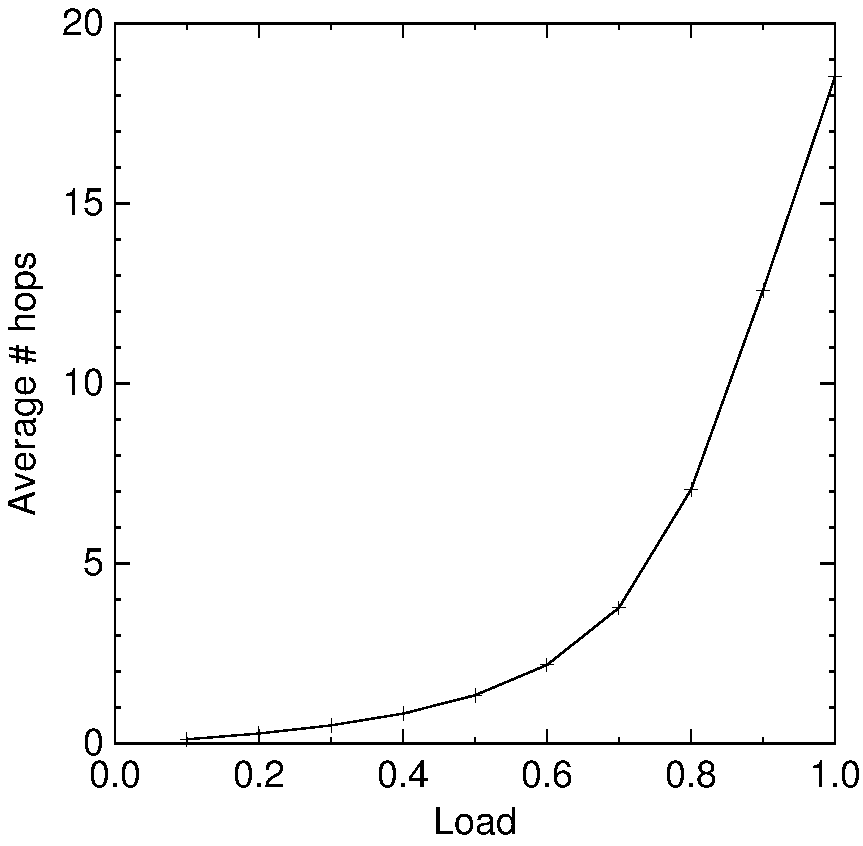
\includegraphics[width=0.6\textwidth]{data/right.pdf}
\caption{The Forward Right baseline result}
\label{baseline}
\end{figure}

All results are obtained using a ring size of 100 and random seeds.


\subsection{Forward to neighbour}

\subsubsection{Left/Right Forward}
It is intuitivly clear that alternating the direction of incoming jobs distributes the load slightly better than keeping the same direction. The performance measure is better than the baseline result for every load level (figure \ref{figlr}). But the improvement is most clear below $0.8$.

\begin{figure}[h!tb]
\centering
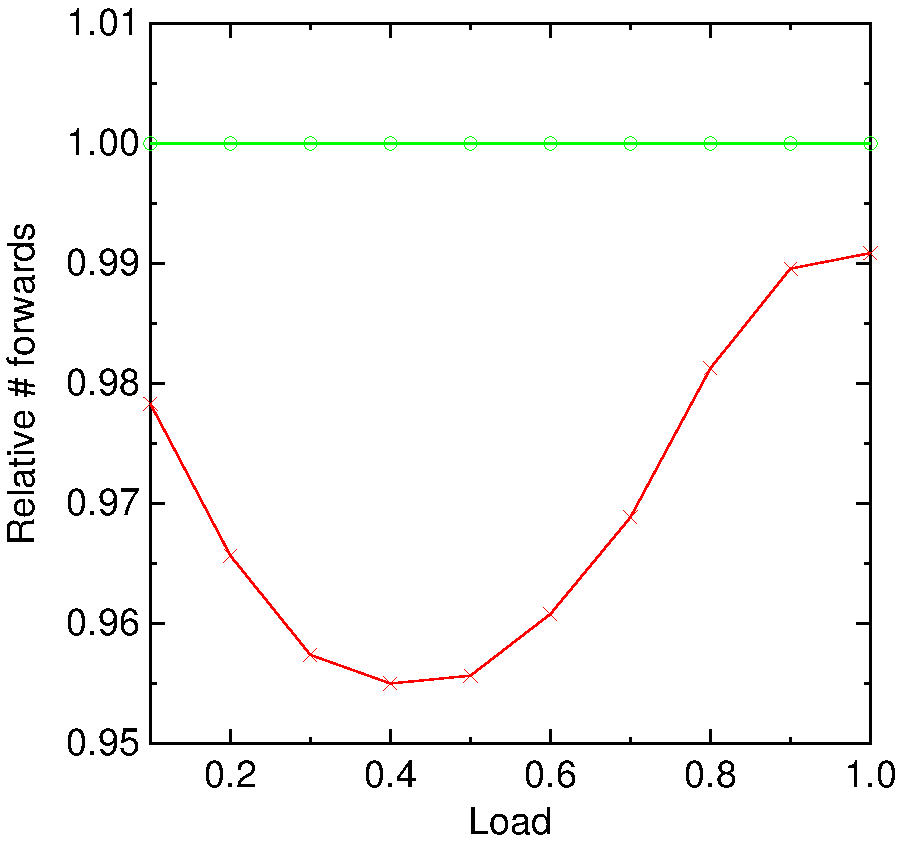
\includegraphics[width=0.6\textwidth]{data/switchright.pdf}
\caption{Left/Right}
\label{figlr}
\end{figure}

\subsubsection{Random Left/Right forward with parameter $p$}
For $p=0.5$, this technique is similar to the previous one. Thus one would expect similar results. However, the results (figure \ref{figrandswitch}) are even worse than our baseline results.

\begin{figure}[h!tb]
\centering
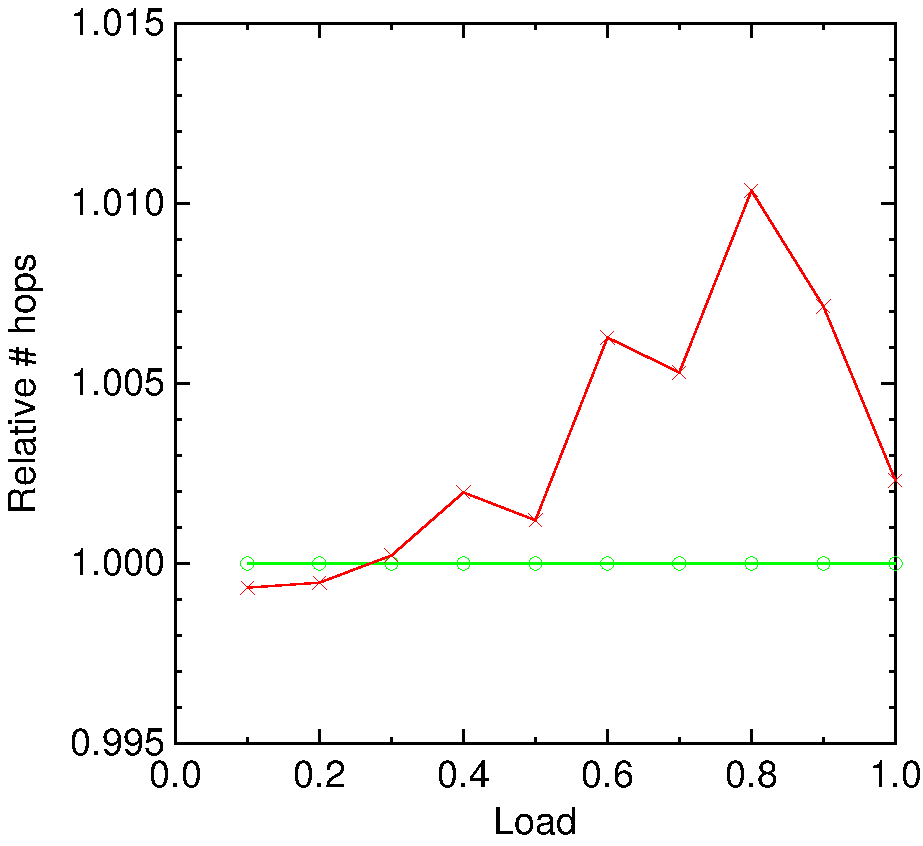
\includegraphics[width=0.6\textwidth]{data/randswitchright.pdf}
\caption{Random Left/Right forward with parameter $0.5$}
\label{figrandswitch}
\end{figure}

This results raises the question how much the parameter influences this result. Since for $p=0$, the algorithm is equal to the Forward Right technique and for $p=0.5$ the results are measurable worse. We will look further into this in section %insert section here%.

\subsubsection{Position-dependant forwarding}
This technique groups nodes in virtual clusters. When a job arrives in a node and that node is busy, the job will be forwarded to the other node in the cluster. Jobs leaving a cluster will do this in a random direction ($p=0.5$). Since the load is concentrated per cluster instead of being distributed over the whole system, this technique performs worse than other techniques The results are represented in figure \ref{figevenswitch}.

\begin{figure}[h!tb]
\centering
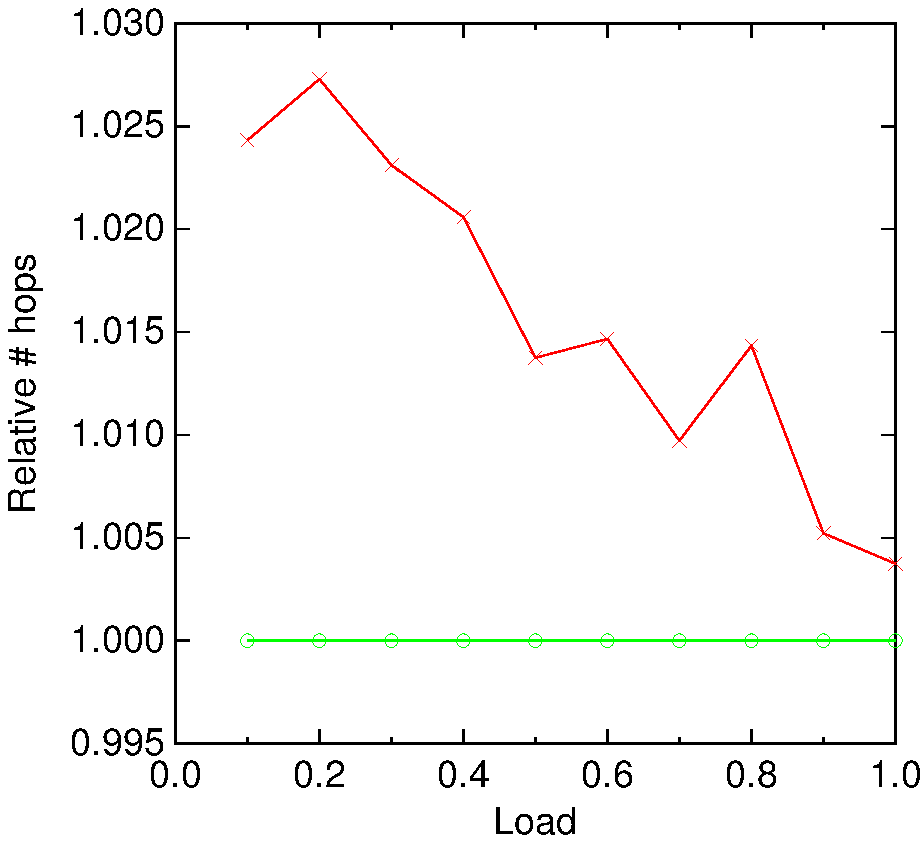
\includegraphics[width=0.6\textwidth]{data/evenswitchright.pdf}
\caption{Position-dependant forwarding}
\label{figevenswitch}
\end{figure}


\subsection{Forward anywhere}

\subsubsection{Random unvisited}
This algorithm in the most straight forward and is the best performing from any of these techniques. However, it should be noted that each visited node must be stored into the job's metadata.

\section{Numerical Validation}
\label{secvalidation}
To validate the results obtained in the previous section, we modelled the scheduling-techniques into Markov Chains. Using the steady state distribution of these chains, we can derive the average number of hops and the average loss. For $N$ nodes in a ring, the markov chain consists of $2^N$ number of states, where the bits represent whether a server is busy or idle. To optimize the computation time and memory requirements, we used sparse matrixes for the validation. The validation code is written in MATLAB.

\subsection{Forward Right}
\label{validateright}
As for this technique, the matrix representing the Markov chain is easily determined. The example given below is for a ring of 3 nodes. For convenience, the states are representes by their binary form.

\[ Q =
  \begin{blockarray}{ccccccccc}
    & 000 & 001 & 010 & 011 & 100 & 101 & 110 & 111 \\
    \begin{block}{c[cccccccc]}
    000 & -3 \lambda & \lambda & \lambda & 0 & \lambda & 0 & 0 & 0 \\
    001 & \mu & -3\lambda-\mu & 0 & \lambda & 0 & 2\lambda & 0 & 0 \\
    010 & \mu & 0 & -3\lambda-\mu & 2\lambda & 0 & 0 & \lambda & 0 \\
    011 & 0 & \mu & \mu & -3\lambda-2\mu & 0 & 0 & 0 & 3\lambda \\
    100 & \mu & 0 & 0 & 0 & -3\lambda-\mu & \lambda & 2\lambda & 0 \\
    101 & 0 & \mu & 0 & 0 & \mu & -3\lambda-2\mu & 0 & 3\lambda \\
    110 & 0 & 0 & \mu & 0 & \mu & 0 & -3\lambda-2\mu & 3\lambda \\
    111 & 0 & 0 & 0 & \mu & 0 & \mu & \mu & -3\mu \\
    \end{block}
  \end{blockarray}
\]

%Include graph here

Analogue to the simulation section, this method will be the baseline result in our other results.

\subsection{Random Left/Right forward with parameter $p$}
This matrix is very similar to the one above. But we need to take into account the parameters $p$ and $1-p$ instead of $1$ and $0$.

\[ Q =
  \begin{blockarray}{ccccccccc}
    & 000 & 001 & 010 & 011 & 100 & 101 & 110 & 111 \\
    \begin{block}{c[cccccccc]}
    000 & -3 \lambda & \lambda & \lambda & 0 & \lambda & 0 & 0 & 0 \\
    001 & \mu & -3\lambda-\mu & 0 & (2-p)\lambda & 0 & (1+p)\lambda & 0 & 0 \\
    010 & \mu & 0 & -3\lambda-\mu & (1+p)\lambda & 0 & 0 & (2-p)\lambda & 0 \\
    011 & 0 & \mu & \mu & -3\lambda-2\mu & 0 & 0 & 0 & 3\lambda \\
    100 & \mu & 0 & 0 & 0 & -3\lambda-\mu & (2-p)\lambda & (1+p)\lambda & 0 \\
    101 & 0 & \mu & 0 & 0 & \mu & -3\lambda-2\mu & 0 & 3\lambda \\
    110 & 0 & 0 & \mu & 0 & \mu & 0 & -3\lambda-2\mu & 3\lambda \\
    111 & 0 & 0 & 0 & \mu & 0 & \mu & \mu & -3\mu \\
    \end{block}
  \end{blockarray}
\]

The lumped matrix of $Q$ is equal to the lumped matrix of the example above (\ref{lump}), i.e. the matrix defines the exact same problem. However, for $N > 6$ the matrices and so the results of the steady state distribution begin to differ.

%Include relative graph here

\subsection{Random Coprime offset}
Modelling this technique yields different results for various ring sizes. The performance of this algorithm is very dependant on the number of coprimes that can be used. This technique yields the same results as Forward Right for ring sizes of up 4. For $N = 3$, the matrix $Q$ is identical to Random Left/Right forward with parameter $0.5$, as the coprimes of 3 are 1 and 2. Which means forwarding a job left or right, both with the same probability.


\subsection{Random Unvisited}
This problem can be modelled much more efficiently than the techniques above. Since the next node is choosen randomly, the information we need to save consists only of the number of servers which are currently busy. This problem is analogue to modelling an Erlang-B loss system. The number of states in this Markov Chain is linear to $N$ and is much more dense. For $N=3$, the matrix is given below.

\[ Q =
  \begin{blockarray}{ccccc}
    & 0 & 1 & 2 & 3 \\
    \begin{block}{c[cccc]}
    0 & -3\lambda & 3\lambda & 0 & 0 \\
    1 & \mu & -3\lambda-\mu & 3\lambda & 0 \\
    2 & 0 & \mu & -3\lambda-\mu & 3\lambda \\
    3 & 0 & 0 & \mu & -\mu \\
    \end{block}
  \end{blockarray}
\]

\subsection{Lumped states}
\label{lump}

Except for Random Unvisited, each discribed technique is modelled into a matrix with $N^2$ states. However, may of these states are redundant: for example, for $N=3$ the states $001$, $010$ and $100$ all represent one of the nodes being busy. For states where multiple nodes are busy, the space between these servers is critical information, therefor states are lumped when rotating the bits of one state becomes equal to another state. The states below are analogue and can be lumped:
\begin{verbatim}
001101 = 011010 = 110100 = 101001 = 010011 = 100110
\end{verbatim}

The number of states in a lumped MC is $\frac{1}{N} \sum_{d|N} (2^{N/d} \cdot phi(d) )$ with $phi(d) = d \cdot \prod_{p|d, p\text{ is prime}} (1-\frac{1}{p})$ \cite{A000031}. This result greatly reduces the number of states, however its complexity is still non-polynomial.

The example model in \ref{validateright} can be lumped into the following Markov Chain:

\[ Q =
  \begin{blockarray}{ccccc}
    & 000 & 001 & 011 & 111 \\
    \begin{block}{c[cccc]}
    000 & -3\lambda & 3\lambda & 0 & 0 \\
    001 & \mu & 3\lambda-\mu & 3\lambda & 0 \\
    011 & 0 & 2\mu & 3\lambda-2\mu & 3\lambda \\
    111 & 0 & 0 & 3\mu & -3\mu \\
    \end{block}
  \end{blockarray}
\]



\subsection{Equivalent techniques}
Lumping states of a Markov Chain produces an equivalent Markov Chain. This can be used to prove some forwarding techniques are equal up to a certain $N$.

\section{Conclusion}
Which techniques work best in which environments? Why? Runner up? Why do some techniques don't work as expected?

\section*{Acknowledgements}
Thanks to everyone

\printbibliography

\appendix
\section{Simulator source code}
\label{sourcecode}
dit is de inhoud

\section{MATLAB Numerical evaluation code}
\label{matlabcode}

\lstset{caption={rightchain.m}}
\lstinputlisting{../matlab/rightchain.m}

\lstset{caption={randswitchchain.m}}
\lstinputlisting{../matlab/randswitchchain.m}

\lstset{caption={rprimechain.m}}
\lstinputlisting{../matlab/rprimechain.m}

\lstset{caption={runvisitedchain.m}}
\lstinputlisting{../matlab/runvisitedchain.m}

\lstset{caption={avghops.m}}
\lstinputlisting{../matlab/avghops.m}

\lstset{caption={ruavghops.m}}
\lstinputlisting{../matlab/ruavghops.m}

\lstset{caption={ctmcsteadystate.m}}
\lstinputlisting{../matlab/ctmcsteadystate.m}

\lstset{caption={lumpavghops.m}}
\lstinputlisting{../matlab/lumpavghops.m}

\lstset{caption={lump.m}}
\lstinputlisting{../matlab/lump.m}

\lstset{caption={makestates.m}}
\lstinputlisting{../matlab/makestates.m}

\end{document}